\documentclass{article}
\usepackage[utf8]{inputenc}
\usepackage{hyperref}
\usepackage{listings}
\usepackage{multimedia} % to embed movies in the PDF file
\usepackage{graphicx}
\usepackage{comment}
\usepackage[english]{babel}
\usepackage{amsmath}
\usepackage{amsfonts}
\usepackage{wrapfig}
\usepackage{multirow}
\usepackage{verbatim}
\usepackage{float}
\usepackage{cancel}
\usepackage{caption}
\usepackage{subcaption}
\usepackage{mathdots}
\usepackage{/home/cade/Homework/latex-defs}


\title{AMATH 574 Homework 1}
\author{Cade Ballew \#2120804}
\date{January 17, 2023}

\begin{document}
	
\maketitle
	
\section{Problem 1}
\subsection{Part a}
Starting from (2.38)
\begin{equation*}
	\begin{split}
		\rho_t + (\rho u)_x &= 0,\\
		(\rho u)_t + (\rho u^2+P(\rho))_x &= 0,
	\end{split} 
\end{equation*} we wish to derive the following nonlinear equations for the pressure and velocity:
\begin{equation*}
	\begin{split}
		p_t + up_x + \rho P'(\rho) u_x &= 0,\\
		u_t + (1/\rho)p_x + uu_x &= 0.
	\end{split} 
\end{equation*}
To derive the first equation, we start we start with the conservation law for $\rho_t$ and multiply through by $P'(\rho)$ to get that
\[
P'(\rho)\rho_t + P'(\rho)\rho_xu+P'(\rho)\rho u_x=0.
\]
Now, we note that  $p_x=P(\rho)_x = P'(\rho)\rho_x,p_t=P(\rho)_t = P'(\rho)\rho_t$, so this can be rewritten as 
\[
p_t+p_xu+\rho P'(\rho)u_x=0,
\]
the first equation. To get the second equation, we expand the conservation law for momentum and substitute $p=P(\rho)$ to get that
\[
\rho_tu+\rho u_t+\rho_xu^2+2\rho uu_x+p_x=0
\] 
which can be further simplified to
\[
\rho_tu+\rho u_t+u(\rho u)_x+\rho uu_x+p_x=0.
\]
Now we plug in the conservation law for $\rho_t$ to get that 
\[
0=-(\rho u)_xu+\rho u_t+u(\rho u)_x+\rho uu_x+p_x=\rho u_t+\rho uu_x+p_x.
\]
Dividing through by $\rho$, this yields the second equation
\[
u_t + (1/\rho)p_x + uu_x = 0.
\]
\subsection{Part b}
To write our system from part a in the form 
\[
q_t(x,t) + A(q(x,t)) q_x(x,t) = 0,
\]
we define 
\[
q=\begin{pmatrix}
	p\\u
\end{pmatrix}
\]
from which we can see that 
\[
\begin{pmatrix}
	p\\u
\end{pmatrix}_t+\begin{pmatrix}
u &\rho P'(\rho)\\1/\rho &u
\end{pmatrix}\begin{pmatrix}
p\\u
\end{pmatrix}_x=0.
\]
Thus, this form can be achieved with this choice of $q$ and 
\[
A(q)=\begin{pmatrix}
	q^{(2)} &\rho P'(\rho)\\1/\rho &q^{(2)}.
\end{pmatrix}
\]
%Using the following Mathematica code, 
%\begin{lstlisting}[language=Mathematica]
%	A = {{u, \[Rho]*Pprime[\[Rho]]}, {1/\[Rho], u}};
%	Eigenvalues[A] // FullSimplify
%	Eigenvectors[A]
%\end{lstlisting}
Using Mathematica, we find that $A(q)$ has eigenvalues $q^{(2)}\pm\sqrt{P'(\rho)}$. 
%\[
%\begin{pmatrix}
%	\pm\rho\sqrt{P'(\rho)}\\1
%\end{pmatrix}.
%\]
This means that $A(q)$ is real diagonalizable iff $P'(\rho)>0$. Note that this matches the condition (2.37) assuming that $\rho>0$.  	
 
\section{Problem 2.7}
Consider the p-system (2.108)
\begin{align*}
v_t-u_x=0,\\
u_t+p(v)_x=0.
\end{align*}
To determine whether this system is hyperbolic, we set
\[
q= \begin{pmatrix}
	v\\u
\end{pmatrix}
\]
which in conjunction with the chain rule allows us to write our system as
\[
\begin{pmatrix}
	v\\u
\end{pmatrix}_t+\begin{pmatrix}
0 &-1\\
p'(v) &0
\end{pmatrix}\begin{pmatrix}
v\\u
\end{pmatrix}_x,
\]
meaning that our system is hyperbolic is hyperbolic if the matrix 
\[
\begin{pmatrix}
	0 &-1\\
	p'(v) &0
\end{pmatrix}
\]
is diagonalizable. Using Mathematica, we find that it has eigenvalues given by $\pm\sqrt{-p'(v)}$, so our system is diagonalizable if $\sqrt{-p'(v)}$ is real for all $v$. Of course, this is true if $p'(v)<0$ for all $v$, so it must hold that our system is hyperbolic if $p'(v)<0$ for all $v$.

\section{Problem 2.8}
Consider isothermal flow modeled by the system (2.38) with $P(\rho)=a^2\rho$ where $a$ is constant. 
\subsection{Part a}
We wish to determine the wave speeds of the linearized equations (2.50)
\[
\begin{pmatrix}
	p\\u
\end{pmatrix}_t+\begin{pmatrix}
	u_0 &K_0\\1/\rho_0 &u_0
\end{pmatrix}\begin{pmatrix}
	p\\u
\end{pmatrix}_x=0
\]
where $K_0=\rho_0P'(\rho_0)$. Note that this is essentially the same system we encountered in problem 1, so we know that the eigenvalues of our matrix are given by $u_0\pm\sqrt{P'(\rho)}$. Plugging in our specific $P$, we get that $P'(\rho)=a^2$, so the wave speeds are given by $u_0\pm a$.
\subsection{Part b}
Consider the p-system (2.107)
\begin{align*}
V_t-U_\xi=0,\\
U_t+p(V)_\xi=0.
\end{align*}
We wish to linearize this system around $V_0,U_0$ in the case where $p(V)=a^2/V$. To do this, we let
\begin{align*}
V=V_0+\Tilde V(x,t),\\
U=U_0+\Tilde U(x,t).
\end{align*}
Plugging this into our system,  we find that 
\begin{align*}
\Tilde V_t-\Tilde U_\xi=0,\\
\Tilde U_t+\left(\frac{a}{V_0+\Tilde V}\right)_\xi=0.
\end{align*}
We drop product terms by noting that 
\[
\frac{1}{V_0+\Tilde{V}}=\frac{1/V_0}{1-\left(-\Tilde{V}/V_0\right)}=\frac{1}{V_0}\sum_{j=0}^{\infty}\left(-\frac{\Tilde V}{V_0}\right)^j=\frac{1}{V_0}-\frac{1}{V_0^2}\Tilde{V}+\frac{1}{V_0^3}\Tilde{V}^2-\ldots
\]
for a sufficiently small perturbation, so
\[
\left(\frac{a^2}{V_0+\Tilde V}\right)_\xi\approx-\frac{a^2}{V_0^2}\Tilde{V}_\xi,
\]
and our linearized system is given by
\[
\begin{pmatrix}
\Tilde{V}\\\Tilde{U}
\end{pmatrix}_t=\begin{pmatrix}
0 &-1\\
-a^2/V_0^2 &0
\end{pmatrix}\begin{pmatrix}
\Tilde{V}\\\Tilde{U}
\end{pmatrix}_\xi.
\]
Using Mathematica, we find that the eigenvalues of the matrix in this system are given by $\pm a/V_0$ which are the Lagrangian wave speeds. To verify that these are what we expect in relation to the Eulerian wave speeds, we note that the relation (2.102) is roughly $\xi = (x-x_0)/V_0$ when linearizing, so $V_0d\xi=dx$, and $V_\xi=V_0V_x$, $U_\xi=V_0U_x$. Thus, the system can be rewritten as 
\[
\begin{pmatrix}
	\Tilde{V}\\\Tilde{U}
\end{pmatrix}_t=\begin{pmatrix}
	0 &-V_0\\
	-a^2/V_0 &0
\end{pmatrix}\begin{pmatrix}
	\Tilde{V}\\\Tilde{U}
\end{pmatrix}_x.
\]
Using Mathematica, we find that the matrix in this system has eigenvalues $\pm a$ which now matches up to the initial velocity $u_0$ as expected.

\section{Problem 3.1}
Using the code from problem 3.2, we provide phase plane plots for the following Riemann problems. 
\subsection{Part d}
\[
A=\begin{pmatrix}
	1&1\\1&1
\end{pmatrix},\quad q_l=\begin{pmatrix}
1\\0
\end{pmatrix},\quad q_r=\begin{pmatrix}
2\\0
\end{pmatrix}
\]
yields the following phase plot\\
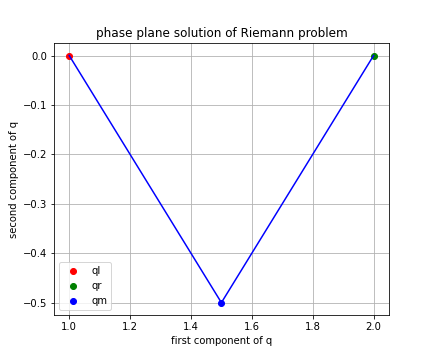
\includegraphics[scale=0.7]{partd.png}\\
and the following solution plots at time $t=1$.\\
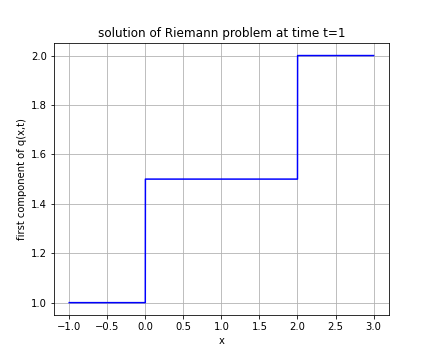
\includegraphics[scale=0.7]{partd1.png}\\
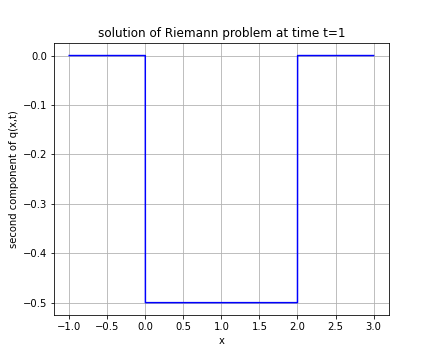
\includegraphics[scale=0.7]{partd2.png}\\
\subsection{Part e}
\[
A=\begin{pmatrix}
	2&0\\0&2
\end{pmatrix},\quad q_l=\begin{pmatrix}
	0\\1
\end{pmatrix},\quad q_r=\begin{pmatrix}
	1\\0
\end{pmatrix}
\]
yields the following phase plot\\
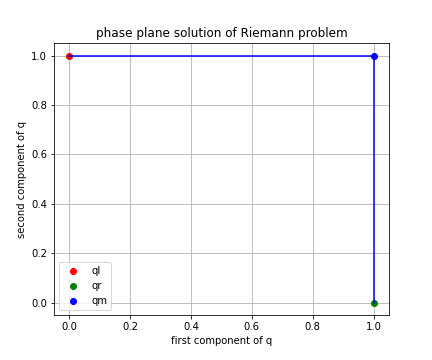
\includegraphics[scale=0.7]{parte.png}
\\
and the following solution plots at time $t=1$.\\
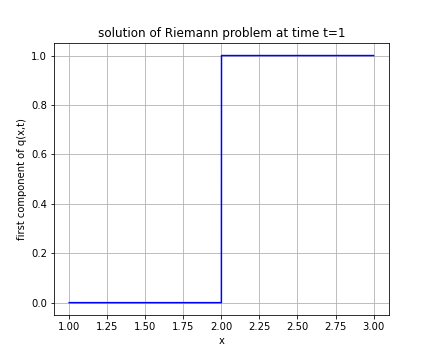
\includegraphics[scale=0.7]{parte1.png}\\
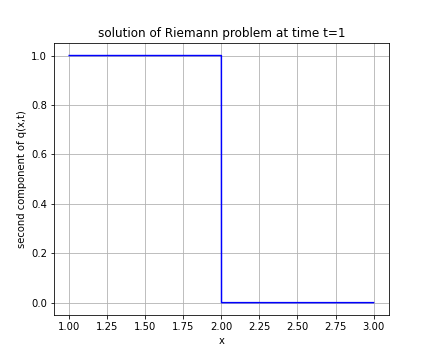
\includegraphics[scale=0.7]{parte2.png}\\
\subsection{Part f}
\[
A=\begin{pmatrix}
	2&1\\10^{-4}&2
\end{pmatrix},\quad q_l=\begin{pmatrix}
	0\\1
\end{pmatrix},\quad q_r=\begin{pmatrix}
	1\\0
\end{pmatrix}
\]
yields the following phase plot\\
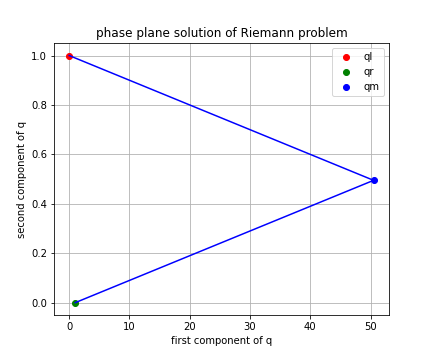
\includegraphics[scale=0.7]{partf.png}\\
and the following solution plots at time $t=1$.\\
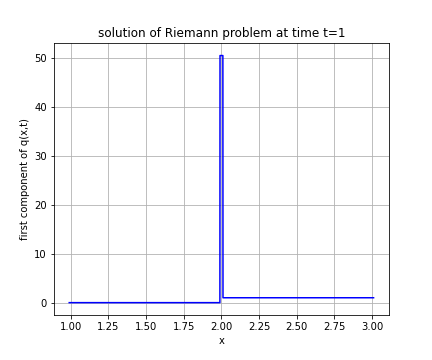
\includegraphics[scale=0.7]{partf1.png}\\
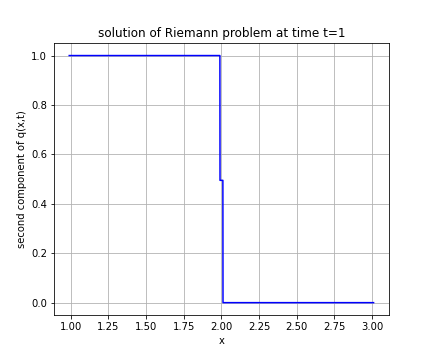
\includegraphics[scale=0.7]{partf2.png}\\

\section{Problem 3.2}
See the attached Jupyter notebook for code which solve $2\times 2$ Riemann problems and produces their phase and solution plots.

\section{Problem 3.3}
\subsection{Part a}
We wish to solve the Riemann problem with 
\[
A=\begin{pmatrix}
	0&0&4\\0&1&0\\1&0&0
\end{pmatrix},\quad q_l=\begin{pmatrix}
	1\\2\\0
\end{pmatrix},\quad q_r=\begin{pmatrix}
	1\\5\\1
\end{pmatrix}.
\]
Using Mathematica, we find that $A$ has eigenvalues $\lambda^1=-2,\lambda^2=1,\lambda^3=2$ with corresponding eigenvectors
\[
r^1=\begin{pmatrix}
	-2\\0\\1
\end{pmatrix},\quad r^2=\begin{pmatrix}
	0\\1\\0
\end{pmatrix},\quad r^3=\begin{pmatrix}
	2\\0\\1
\end{pmatrix},
\]
so we set 
\[
R=\begin{pmatrix}
	-2&0&2\\	
	0&1&0\\
	1&0&1
\end{pmatrix}
\]
and solve the linear system 
\[
R\alpha=q_r-q_l=\begin{pmatrix}
	0\\3\\1
\end{pmatrix}
\]
via Mathematica to get
\[
\alpha=\begin{pmatrix}
	1/2\\3\\1/2
\end{pmatrix}.
\]
From this, we can compute $q$ at our two middle states as follows.
\begin{align*}
q_{l}^*=q_l+\alpha^1r^1=\begin{pmatrix}
	1\\2\\0
\end{pmatrix}+\frac{1}{2}\begin{pmatrix}
-2\\0\\1
\end{pmatrix}=\begin{pmatrix}
0\\2\\1/2
\end{pmatrix},\\
q_{r}^*=q_r-\alpha^3r^3=\begin{pmatrix}
	1\\5\\1
\end{pmatrix}-\frac{1}{2}\begin{pmatrix}
2\\0\\1
\end{pmatrix}=\begin{pmatrix}
0\\5\\1/2
\end{pmatrix}.
\end{align*}
We include the following (crude) sketch of the regions in which each state is valid.
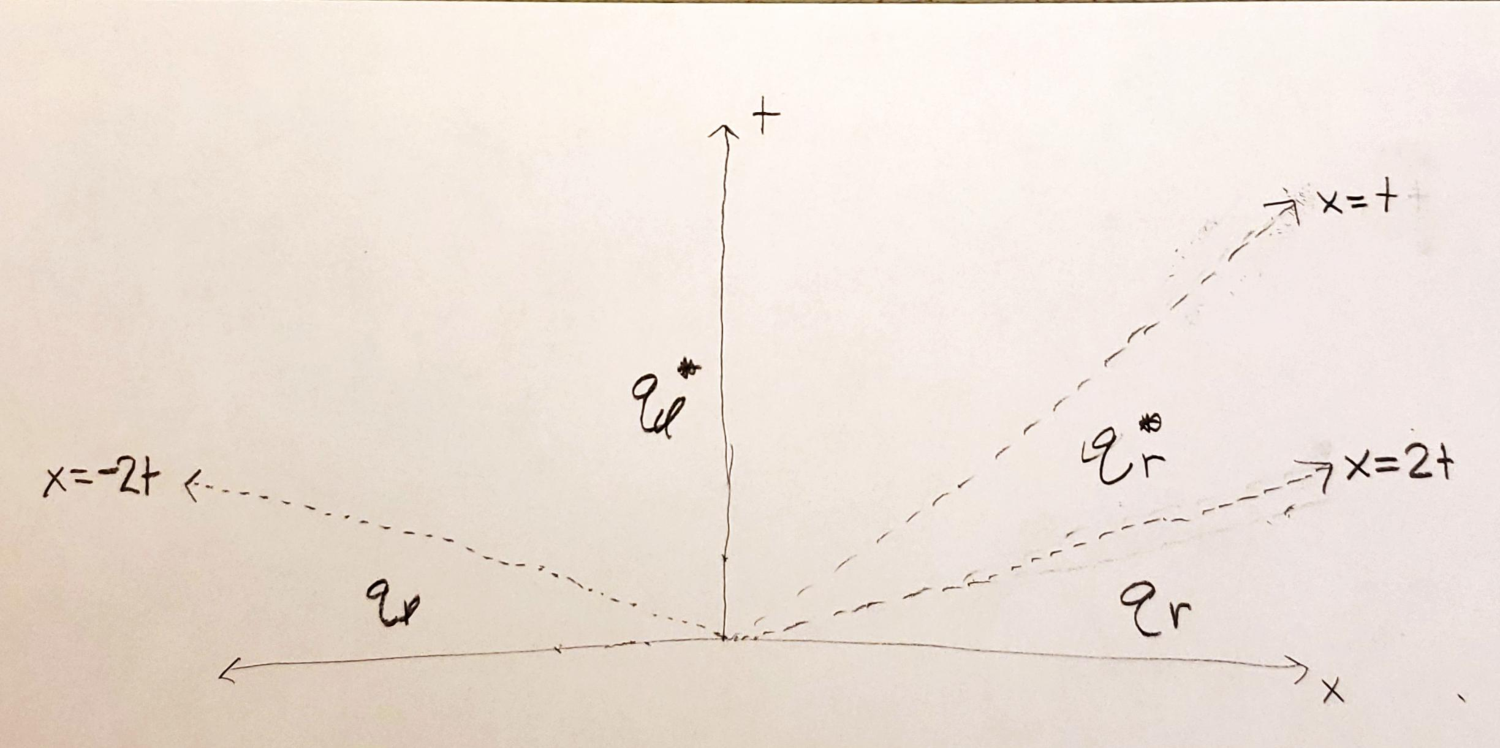
\includegraphics[scale=0.5]{574hw1figs-1.pdf}

\subsection{Part b}
We wish to solve the Riemann problem with 
\[
A=\begin{pmatrix}
	1&0&2\\0&2&0\\0&0&3
\end{pmatrix},\quad q_l=\begin{pmatrix}
	1\\1\\1
\end{pmatrix},\quad q_r=\begin{pmatrix}
	3\\3\\3
\end{pmatrix}.
\]
Using Mathematica, we find that $A$ has eigenvalues $\lambda^1=1,\lambda^2=2,\lambda^3=3$ with corresponding eigenvectors
\[
r^1=\begin{pmatrix}
	1\\0\\0
\end{pmatrix},\quad r^2=\begin{pmatrix}
	0\\1\\0
\end{pmatrix},\quad r^3=\begin{pmatrix}
	1\\0\\1
\end{pmatrix},
\]
so we set
\[
R=\begin{pmatrix}
	1&0&1\\
	0&1&0\\
	0&0&1
\end{pmatrix}
\]
and solve the linear system 
\[
R\alpha=q_r-q_l=\begin{pmatrix}
	2\\2\\2
\end{pmatrix}
\]
via Mathematica to get
\[
\alpha=\begin{pmatrix}
	0\\2\\2
\end{pmatrix}.
\]
From this, we can compute $q$ at our two middle states as follows.
\begin{align*}
q_{l}^*=q_l+\alpha^1r^1=\begin{pmatrix}
	1\\1\\1
\end{pmatrix}-0\begin{pmatrix}
1\\0\\0
\end{pmatrix}=\begin{pmatrix}
1\\1\\1
\end{pmatrix},\\
q_r^*=q_r-\alpha^3r^3=\begin{pmatrix}
	3\\3\\3
\end{pmatrix}-2\begin{pmatrix}
1\\0\\1
\end{pmatrix}=\begin{pmatrix}
1\\3\\1
\end{pmatrix}.
\end{align*}
We include the following sketch of the regions in which each state is valid. Note that $q_l=q_l^*$ so we really only have three states.\\
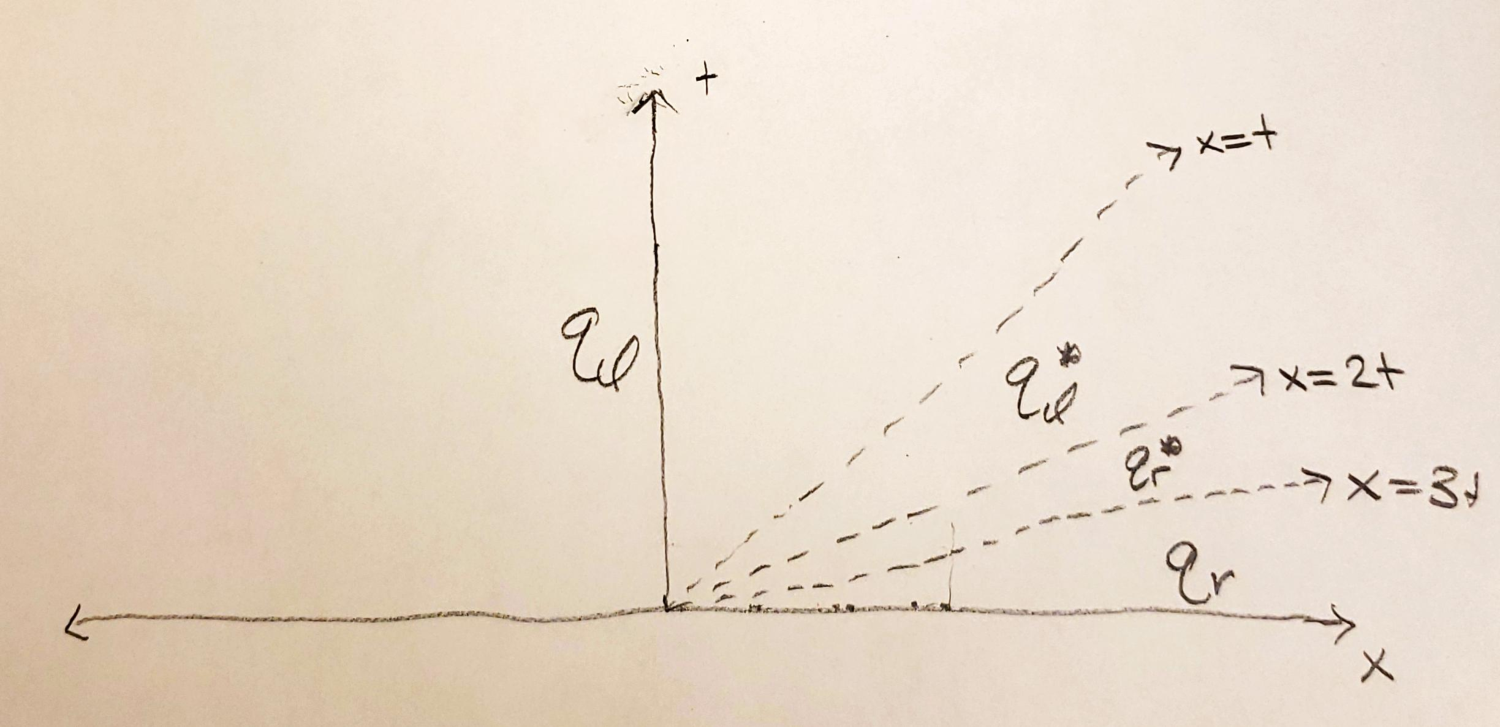
\includegraphics[scale=0.5]{574hw1figs-2.pdf}
\end{document}
